\documentclass[a4paper,12pt,french]{article}

\usepackage[cours]{../../../Style}

\pgfplotsset{styleglobal/.append style={xlabel={$n$}}}

% Début du document
%%%%%%%%%%%%%%%%%%%
\begin{document}

\title{Suites arithmétiques et géométriques}
\maketitle

\begin{programme}
\item Suites arithmétiques: évolutions absolues constantes (croissance linéaire).
\item Suites géométriques: évolutions relatives constantes (croissance exponentielle).
\begin{itemize}
\item Relation de récurrence
\item Sens de variation
\item Représentation graphique
\end{itemize}
\item Compétences
\begin{itemize}
\item Reconnaitre si une situation relève d'un modèle discret de croissance linéaire ou exponentielle.
\item Conjecturer, à partir de sa représentation graphique, la nature arithmétique ou géométrique d'une suite.
\item Démontrer qu'une suite est arithmétique ou géométrique.
\item Déterminer le sens de variation d'une suite arithmétique ou géométrique à l'aide de la raison.
\end{itemize}
\end{programme}

\section{Suites arithmétiques}

\subsection{Généralités}

\begin{defin}
Une suite est dite arithmétique lorsque l'on passe d'un terme au suivant en ajoutant toujours le même nombre, appelé la raison. 

Pour définir une suite arithmétique $a$, on a besoin de deux nombres:
\begin{itemize}
\item Son premier terme $a_0$
\item Sa raison $r$
\end{itemize}
On a alors la relation $a_{n+1}=a_n+r$ pour tout $n \in \N$.

\begin{center}
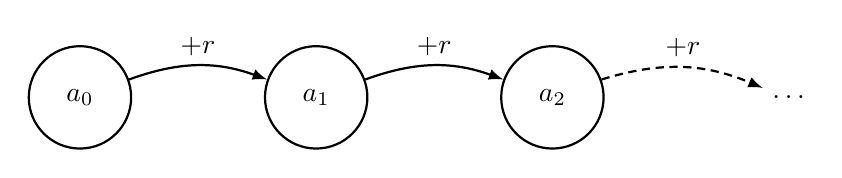
\begin{tikzpicture}[scale=1]
% Fond: fill=white,fill opacity=0.8,text opacity=1
% Ombre portée: fill=white,drop shadow={opacity=0.3}
\node[draw,circle,thick, minimum size=13mm] (W0) at (-3,0) {$a_0$}; 
\node[draw,circle,thick, minimum size=13mm] (W1) at (0,0) {$a_1$};
\node[draw,circle,thick, minimum size=13mm] (W2) at (3,0) {$a_2$};
\node (W5) at (6,0) {$\ldots$};
\draw[->,>=latex,thick] (W0) to[bend left=20] node[midway,above]{$+r$} (W1);
\draw[->,>=latex,thick] (W1) to[bend left=20] node[midway,above]{$+r$} (W2);
\draw[->,>=latex,thick,densely dashed] (W2) to[bend left=20] node[midway,above]{$+r$} (W5);
\end{tikzpicture}
\end{center}

\end{defin}

\begin{ex}
Soit $u$ la suite arithmétique de premier terme $u_0=5$ et de raison $r=-2$. Alors:
$$
\begin{aligned}
u_1&=u_0-2=3\\
u_2&=u_1-2=1\\
u_3&=u_2-2=-1\\
u_4&=\ \ldots
\end{aligned}
$$
\end{ex}

\begin{rmq}
La différence entre deux termes successifs vaut toujours $r$: Pour tout $n \in \N, a_{n+1}-a_n=r$.
\end{rmq}

\rem{Exos 32,(33) p91\\Exos 70,71 p94\\Exos 37,76,(78) p91/94\\Exo 75p94}
\rem{Preuves: Exos 75,77 p94}
\subsection{Représentation graphique}

\begin{propr}
Lorsqu'on représente graphiquement une suite arithmétique, les points obtenus sont alignés.
\end{propr}

\begin{ex}
\begin{center}
\begin{tikzpicture}[scale=\echellepgf]
\begin{axis}[
styleglobal,
hauteurproptick,
width=0.6*\echellepgfinv*\linewidth,
xmin=-0.5, xmax=10.5,
ymin=-2.5, ymax=3.5,
xtick distance=1,
ytick distance=1
]
\addplot[samples=11,domain=(0:10),only marks,semithick,fill=blue]{-0.5*x+3};
%\addplot[styleplot,color=red,domain=(1:2)]{1} \pointsextremites;	%test
%\node[stylepoint,fill=blue,inner sep=1.4pt] at (4.9,0.5) {};		%test
\end{axis}
\end{tikzpicture}
\end{center}

On a représenté une suite arithmétique $u$ ci-dessus. On a $u_0 = 3$ et $u_1=2,5$. Alors $r=u_1-u_0=2,5-3=-0.5$. La suite $u$ est donc une suite arithmétique de premier terme $3$ et de raison $r=-0.5$.
\end{ex}

\rem{Exo 36 p91}

\begin{comment}
\begin{methode}
Pour s'assurer qu'une suite \textbf{semble} arithmétique, on calcule la différence entre deux termes successifs, et l'on doit toujours trouver le même nombre (la raison).
\end{methode}

\begin{ex}
On se donne deux suites $u$ et $v$, dont quelques valeurs sont décrites dans le tableau ci-dessous:
\begin{center}
\begin{tabularx}{0.5\linewidth}{|c|*{4}{Y|}} \hline
$n$ & 0 & 1 & 2 & 3 \\ \hline
$u_n$ & 5 & 9 & 13 & 17 \\ \hline
$v_n$ & 3 & 12 & 20 & 29 \\ \hline
\end{tabularx}
\end{center}
\end{ex}
\end{comment}

\subsection{Variations des suites arithmétiques}

\begin{prop}
\begin{itemize}
\item Si $r > 0$, alors la suite $a$ est croissante.
\item Si $r < 0$, alors la suite $a$ est décroissante.
\item Si $r = 0$, alors la suite $a$ est constante.
\end{itemize}
\end{prop}

\begin{ex}
Soit $a$ la suite arithmétique définie par $a_0=13$ et pour tout $n \in \N, a_{n+1}=a_n-5$. La raison de cette suite est $r=-5<0$ donc $a$ est décroissante.
\end{ex}

\rem{Exo 83 p95}

\section{Suites géométriques, cas positif}

\subsection{Généralités}

\begin{defin}
Une suite est dite géométrique lorsque l'on passe d'un terme au suivant en multipliant toujours par le même nombre, appelé la raison. 

Pour définir une suite géométrique $g$, on a besoin de deux nombres:
\begin{itemize}
\item Son premier terme $g_0$
\item Sa raison $q$
\end{itemize}
On a alors la relation $g_{n+1}=q \times g_n$ pour tout $n \in \N$.

\begin{center}
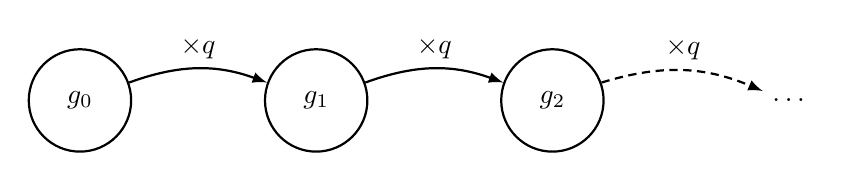
\begin{tikzpicture}[scale=1]
\node[draw,circle,thick, minimum size=13mm] (W0) at (-3,0) {$g_0$};
\node[draw,circle,thick, minimum size=13mm] (W1) at (0,0) {$g_1$};
\node[draw,circle,thick, minimum size=13mm] (W2) at (3,0) {$g_2$};
\node (W5) at (6,0) {$\ldots$};
\draw[->,>=latex,thick] (W0) to[bend left=20] node[midway,above]{$\times q$} (W1);
\draw[->,>=latex,thick] (W1) to[bend left=20] node[midway,above]{$\times q$} (W2);
\draw[->,>=latex,thick,densely dashed] (W2) to[bend left=20] node[midway,above]{$\times q$} (W5);
\end{tikzpicture}
\end{center}
\end{defin}

\rem[eleve]{On se restreindra au cas où $g_0$ et $q$ sont strictement positifs.}

\begin{ex}
Soit $g$ la suite géométrique de premier terme $g_0=3$ et de raison $q=2$. Alors:
$$
\begin{aligned}
g_1&=g_0 \times 2=6\\
g_2&=g_1 \times 2=12\\
g_3&=g_2 \times 2=24\\
g_4&=\ \ldots
\end{aligned}
$$
\end{ex}

\begin{rmq}
Le quotient de deux termes successifs vaut toujours $q$: $\frac{g_{n+1}}{g_n}=q$.
\end{rmq}

\rem{Exos 34,35 p91\\Exos 72,73,(82) p94\\Exo 80p94}
\rem{Preuves: Exos 79,81 p94}

\subsection{Représentation graphique des suites géométriques}

\begin{exs}
\compo{
\begin{centrer}
\textbf{Cas 1: $q > 1$}
\begin{tikzpicture}[scale=\echellepgf]
\begin{axis}[
styleglobal,
hauteurproptick,
width=0.8*\echellepgfinv*\linewidth,
xmin=-0.5, xmax=10.5,
ymin=-100, ymax=1500,
xtick distance=1,
ytick distance=200,
legend style={at={(0.1,0.97)},anchor=north west},
legend cell align=left,
]
\addplot[samples=11,domain=(0:10),only marks,fill=blue,semithick]{1*2^x};
\addplot[samples=11,domain=(0:10),only marks,mark=square*,semithick,fill=red]{60*1.25^x};
\addplot[samples=11,domain=(0:10),only marks,mark=triangle*,semithick,fill=green]{300*1.1^x};
\legend{$u_0=1,\ q=2$\\$v_0=60,\ q=1.25$\\$w_0=300,\ q=1.1$\\} % \\ nécessaire pour que la virgule fonctionne
%\addplot[styleplot,color=red,domain=(1:2)]{1} \pointsextremites;	%test
%\node[stylepoint,fill=blue,inner sep=1.4pt] at (4.9,0.5) {};		%test
\end{axis}
\end{tikzpicture}
\end{centrer}
}
{
\begin{centrer}
\textbf{Cas 2: $0<q<1$}
\begin{tikzpicture}[scale=\echellepgf]
\begin{axis}[
styleglobal,
hauteurproptick,
width=0.8*\echellepgfinv*\linewidth,
xmin=-0.5, xmax=10.5,
ymin=-0.5, ymax=7.5,
xtick distance=1,
ytick distance=1,
legend cell align=left,
]
\addplot[samples=11,domain=(0:10),only marks,semithick,fill=blue]{4*0.5^x};
\addplot[samples=11,domain=(0:10),mark=square*,only marks,semithick,fill=red]{5*0.9^x};
\legend{$v_0=4,\ q=0.5$\\$v_0=5,\ q=0.9$\\}
%\addplot[styleplot,color=red,domain=(1:2)]{1} \pointsextremites;	%test
%\node[stylepoint,fill=blue,inner sep=1.4pt] at (4.9,0.5) {};		%test
\end{axis}
\end{tikzpicture}
\end{centrer}
}
\end{exs}

\rem{Exo 40p91}

\subsection{Variations des suites géométriques}

\begin{prop}
\begin{itemize}
\item Si $q > 1$, alors la suite $g$ est croissante.
\item Si $0< q < 1$, alors la suite $g$ est décroissante.
\item Si $q = 1$, alors la suite $g$ est constante.
\end{itemize}
\end{prop}

\begin{ex}
Soit $g$ la suite géométrique définie par $g_0=5$ et pour tout $n \in \N, g_{n+1}=0,9 \times g_n$. La raison de cette suite est $q=0,9 < 1$ donc $g$ est décroissante.
\end{ex}

\rem{Exo 84 p95}

\rem{Exo 74 p94\\Exo 94 p96\\Exos 86,88 p95}

\begin{comment}
\begin{ex}
\compo{
\begin{center}
\begin{tikzpicture}[scale=\echellepgf]
\begin{axis}[
styleglobal,
hauteurproptick,
width=0.9*\echellepgfinv*\linewidth,
xmin=-0.5, xmax=10.5,
ymin=-0.5, ymax=1050,
xtick distance=1,
ytick distance=100,
legend style={at={(0.1,0.97)},anchor=north west},
]
\addplot[samples=11,domain=(0:10),only marks,stylepoint,fill=blue]{1*2^x};
\addlegendentry{$u_0=1, q=2$};
%\addplot[styleplot,color=red,domain=(1:2)]{1} \pointsextremites;	%test
%\node[stylepoint,fill=blue,inner sep=1.4pt] at (4.9,0.5) {};		%test
\end{axis}
\end{tikzpicture}
\end{center}
}
{
\begin{center}
\begin{tikzpicture}[scale=\echellepgf]
\begin{axis}[
styleglobal,
hauteurproptick,
width=0.9*\echellepgfinv*\linewidth,
xmin=-1, xmax=10.5,
ymin=-0.5, ymax=3.5,
xtick distance=1,
ytick distance=1
]
\addplot[samples=11,domain=(0:10),only marks,stylepoint,fill=blue]{3*0.5^x};
\addlegendentry{$v_0=3, q=0.7$};
%\addplot[styleplot,color=red,domain=(1:2)]{1} \pointsextremites;	%test
%\node[stylepoint,fill=blue,inner sep=1.4pt] at (4.9,0.5) {};		%test
\end{axis}
\end{tikzpicture}

\

\begin{tikzpicture}[scale=\echellepgf]
\begin{axis}[
styleglobal,
hauteurproptick,
width=0.9*\echellepgfinv*\linewidth,
xmin=-1, xmax=10.5,
ymin=-5.5, ymax=0.5,
xtick distance=1,
ytick distance=1,
legend pos=south east,
]
\addplot[samples=11,domain=(0:10),only marks,stylepoint,fill=blue]{-5*0.9^x};
\addlegendentry{$v_0=-5, q=0.9$};
%\addplot[styleplot,color=red,domain=(1:2)]{1} \pointsextremites;	%test
%\node[stylepoint,fill=blue,inner sep=1.4pt] at (4.9,0.5) {};		%test
\end{axis}
\end{tikzpicture}
\end{center}
}
\end{ex}
\end{comment}

\end{document}
